\input{preamble}

\section*{Bloch sphere}

Let $|s\rangle$ be the spin state
\begin{equation*}
|s\rangle=\begin{pmatrix}
\cos(\theta/2)
\\
\sin(\theta/2)\exp(i\phi)
\end{pmatrix}
\end{equation*}

Spin $|s\rangle$ can be visualized as a point on a unit sphere.
% https://diagrams.janosh.dev/bloch-sphere
\begin{center}
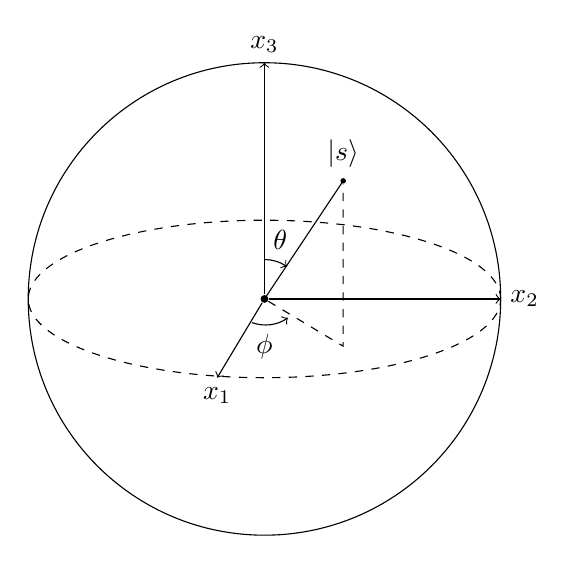
\begin{tikzpicture}

  % Define radius
  \def\r{3}

  % Bloch vector
  % \draw (0, 0) node[circle, fill, inner sep=1] (orig) {} -- (\r/3, \r/2) node[circle, fill, inner sep=0.7, label=above:$\vec{a}$] (a) {};
  \draw (0, 0) node[circle, fill, inner sep=1] (orig) {} -- (\r/3, \r/2) node[circle, fill, inner sep=0.7, label=above:$|s\rangle$] (a) {};
  \draw[dashed] (orig) -- (\r/3, -\r/5) node (phi) {} -- (a);

  % Sphere
  \draw (orig) circle (\r);
  \draw[dashed] (orig) ellipse (\r{} and \r/3);

  % Axes
  \draw[->] (orig) -- ++(-\r/5, -\r/3) node[below] (x1) {$x_1$};
  \draw[->] (orig) -- ++(\r, 0) node[right] (x2) {$x_2$};
  \draw[->] (orig) -- ++(0, \r) node[above] (x3) {$x_3$};

  % Angles
  %\pic [draw=gray, text=gray, ->, "$\phi$"] {angle = x1--orig--phi};
  %\pic [draw=gray, text=gray, <-, "$\theta$", angle eccentricity=1.4] {angle = a--orig--x3};

\draw[->] (0,0.5) arc[start angle=90, end angle=55, radius=0.5];
\node[black] at (0.2,0.75) {$\theta$};

\draw[->] (-0.16,-0.3) arc[start angle=-110, end angle=-55, radius=0.5];
\node at (0,-0.6) {$\phi$};

\end{tikzpicture}
\end{center}

Start with an arbitrary complex vector $|\chi\rangle$ such that $\langle\chi|\chi\rangle=1$.
\begin{equation*}
|\chi\rangle
=\begin{pmatrix}
A\exp(i\phi_1)
\\
\sqrt{1-A^2}\exp(i\phi_2)
\end{pmatrix}
\end{equation*}

Let $|s\rangle$ be the spin
\begin{equation*}
|s\rangle=\exp(-i\phi_1)|\chi\rangle
=\begin{pmatrix}
A
\\
\sqrt{1-A^2}\exp[i(\phi_2-\phi_1)]
\end{pmatrix}
\end{equation*}

Substitute $\cos(\theta/2)$ for $A$ and $\sin(\theta/2)$ for $\sqrt{1-A^2}$.
\begin{equation*}
|s\rangle=\begin{pmatrix}
\cos(\theta/2)
\\
\sin(\theta/2)\exp[i(\phi_2-\phi_1)]
\end{pmatrix}
\end{equation*}

By equality of expectation values $|\chi\rangle$ and $|s\rangle$ are representations of the same spin.
\begin{align*}
\langle S_x\rangle=\langle\chi|S_x|\chi\rangle&=\langle s|S_x|s\rangle
\\
\langle S_y\rangle=\langle\chi|S_y|\chi\rangle&=\langle s|S_y|s\rangle
\\
\langle S_z\rangle=\langle\chi|S_z|\chi\rangle&=\langle s|S_z|s\rangle
\end{align*}

Hence every $|\chi\rangle$ has a place on the Bloch sphere.

\bigskip
\href{https://georgeweigt.github.io/examples/bloch-sphere-demo.html}{Eigenmath script}

\end{document}
